\documentclass[compress]{beamer}
\mode<presentation>
\setbeamercovered{transparent}
\usetheme{Warsaw}
%\useoutertheme{smoothtree}
\usepackage{multirow}
\usepackage[english]{babel}
\usepackage[latin1]{inputenc}
\usepackage{times}
\usepackage[T1]{fontenc}
\usepackage{xmpmulti}
\usepackage{multicol}
\usepackage{colortbl}

%\setbeamersize{text margin left=.25 in,text margin right=.25 in}
\setbeamersize{text margin left=.15 in,text margin right=.15 in}
\usepackage[authoryear]{natbib}


\usepackage{epstopdf}
\usepackage{xcolor}
\usepackage{latexcolors}
%\usepackage[dvipsnames]{xcolor}
\definecolor{antiquebrass}{rgb}{0.8, 0.58, 0.46}
\definecolor{babyblueeyes}{rgb}{0.63, 0.79, 0.95}
\definecolor{babyblue}{rgb}{0.54, 0.81, 0.94}
\definecolor{bistre}{rgb}{0.24, 0.17, 0.12}
\definecolor{brightlavender}{rgb}{0.75, 0.58, 0.89}
\definecolor{bulgarianrose}{rgb}{0.28, 0.02, 0.03}
\definecolor{slateblue}{rgb}{0.56, 0.74, 0.56}
\definecolor{cordovan}{rgb}{0.54, 0.25, 0.27}
\definecolor{darkbyzantium}{rgb}{0.36, 0.22, 0.33}

\setbeamercolor{structure}{fg=airforceblue!80, bg= black!60}







\usepackage{tikz}
\usetikzlibrary{shadows,calc}
\usetikzlibrary{shadows.blur}
\usetikzlibrary{shapes.symbols}
\usepackage{hyperref}
\usepackage{booktabs}
\usepackage{colortbl}
\usepackage{multirow}
%%%%%%%%% shaddow image %%%%%
% some parameters for customization
\def\shadowshift{3pt,-3pt}
\def\shadowradius{6pt}
\colorlet{innercolor}{black!60}
\colorlet{outercolor}{gray!05}
% this draws a shadow under a rectangle node
\newcommand\drawshadow[1]{
\begin{pgfonlayer}{shadow}
    \shade[outercolor,inner color=innercolor,outer color=outercolor] ($(#1.south west)+(\shadowshift)+(\shadowradius/2,\shadowradius/2)$) circle (\shadowradius);
    \shade[outercolor,inner color=innercolor,outer color=outercolor] ($(#1.north west)+(\shadowshift)+(\shadowradius/2,-\shadowradius/2)$) circle (\shadowradius);
    \shade[outercolor,inner color=innercolor,outer color=outercolor] ($(#1.south east)+(\shadowshift)+(-\shadowradius/2,\shadowradius/2)$) circle (\shadowradius);
    \shade[outercolor,inner color=innercolor,outer color=outercolor] ($(#1.north east)+(\shadowshift)+(-\shadowradius/2,-\shadowradius/2)$) circle (\shadowradius);
    \shade[top color=innercolor,bottom color=outercolor] ($(#1.south west)+(\shadowshift)+(\shadowradius/2,-\shadowradius/2)$) rectangle ($(#1.south east)+(\shadowshift)+(-\shadowradius/2,\shadowradius/2)$);
    \shade[left color=innercolor,right color=outercolor] ($(#1.south east)+(\shadowshift)+(-\shadowradius/2,\shadowradius/2)$) rectangle ($(#1.north east)+(\shadowshift)+(\shadowradius/2,-\shadowradius/2)$);
    \shade[bottom color=innercolor,top color=outercolor] ($(#1.north west)+(\shadowshift)+(\shadowradius/2,-\shadowradius/2)$) rectangle ($(#1.north east)+(\shadowshift)+(-\shadowradius/2,\shadowradius/2)$);
    \shade[outercolor,right color=innercolor,left color=outercolor] ($(#1.south west)+(\shadowshift)+(-\shadowradius/2,\shadowradius/2)$) rectangle ($(#1.north west)+(\shadowshift)+(\shadowradius/2,-\shadowradius/2)$);
    \shade[outercolor,right color=innercolor,left color=innercolor] ($(#1.north west)+(-\shadowradius/12,\shadowradius/12)$) rectangle ($(#1.south east)+(\shadowradius/12,-\shadowradius/12)$);%Frame
    \filldraw ($(#1.south west)+(\shadowshift)+(\shadowradius/2,\shadowradius/2)$) rectangle ($(#1.north east)+(\shadowshift)-(\shadowradius/2,\shadowradius/2)$);
\end{pgfonlayer}
}
% create a shadow layer, so that we don't need to worry about overdrawing other things
\pgfdeclarelayer{shadow} 
\pgfsetlayers{shadow,main}
% Define image shadow command
\newcommand\shadowimage[2][]{%
\begin{tikzpicture}
\node[anchor=south west,inner sep=0] (image) at (0,0) {\includegraphics[#1]{#2}};
\drawshadow{image}
\end{tikzpicture}}
\usepackage{calligra}

\DeclareMathOperator*{\argmax}{Arg\,max}
\DeclareMathOperator*{\argmin}{Arg\,min}
\newcommand{\norm}[1]{\left\Vert #1 \right\Vert }
\newcommand{\bbetaHat}{ \widehat{\bbeta}}
\newcommand{\bbetaLSE}{ \widehat{\bbeta}_{_{\text{LSE}}}}
\newcommand{\bbetaMLE}{ \widehat{\bbeta}_{_{\text{MLE}}}}
\newcommand{\sqBullet}[1]{  {\tiny \tiny \tiny \qBoxCol{#1!60}{ }} }
%***************
%\newtheorem{thm}{Theorem}
%\documentclass[noinfoline]{imsart}
%\usepackage{amsmath,amstext,amssymb}
%%\usepackage[top=1.5in, bottom=1.5in, left=1.2in, right=1.2in]{geometry}
%% settings
%%\pubyear{2005}
%%\volume{0}
%%\issue{0}
%%\firstpage{1}
%%\lastpage{8}
%\arxiv{arXiv:0000.0000}

%\startlocaldefs
%\numberwithin{equation}{section}
%\theoremstyle{plain}
%\newtheorem{thm}{Theorem}
%\endlocaldefs
\usepackage{lipsum} 
\usepackage{amsmath}
\usepackage{amssymb}
\usepackage{amsbsy} 
\usepackage{amsthm}
\usepackage{mathrsfs}
\usepackage{eufrak}
\usepackage{mathrsfs}
\usepackage{color}
\usepackage{verbatim}
\usepackage{graphicx}
\usepackage{bm}
\usepackage{enumerate}
\usepackage{epstopdf} 
\usepackage{natbib}
\usepackage{undertilde}
%\RequirePackage[colorlinks,citecolor=blue,urlcolor=blue]{hyperref}
%\usepackage{subfig}
\usepackage[final]{pdfpages}

\usepackage{algorithm}  %@subhajit
\usepackage{algpseudocode} %@subhajit
\usepackage{algorithmicx}     %@subhajit
\usepackage{undertilde}


\newcommand{\sphere}{{\mathbb{S}}}
\newcommand{\R}{\mathbb{R}}
\newcommand{\LatentV}{V}
\newcommand{\NC}{m}
\newcommand{\Priorf}{f_{prior}}
\newcommand{\FWOne}[2]{{{}_{1}\Psi _{1}\left[{\begin{matrix}(\frac{#1}{2},\frac{1}{2})\\(1,0)\end{matrix}};#2\right]} 
}


\newcommand{\HyPriorMu}{\thetabf}
\newcommand{\HyPriorAlpha}{\alpha}
\newcommand{\HyPriorBeta}{\beta}
\newcommand{\HyPriorK}{\zeta}
\newcommand{\Indicator}[2]{\mathbb{I}_{_{#1}}({#2 })}
\newcommand{\xb}{\bm{x}}
\newcommand{\bx}{\MakeVec{\bm{x}}}
\newcommand{\bX}{\bm{X}}
\newcommand{\by}{\MakeVec{\bm{y}}}
\newcommand{\bZ}{\bm{Z}}
\newcommand{\bF}{\bm{F}}
\newcommand{\btheta}{\MakeVec{{\bm{\theta}}}}
\newcommand{\Bpi}{\MakeVec{\boldsymbol{\pi}}}
\newcommand{\thetabf}{\MakeVec{\boldsymbol{\theta}}}
\newcommand{\Thetabf}{\boldsymbol{\Theta}}
\newcommand{\taubf}{\MakeVec{\boldsymbol{\tau}}}
\newcommand{\Tr}{Tr}


\newcommand{\bM}{\bm{M}}
\newcommand{\bD}{\MakeVec{\bm{D}}}
\newcommand{\bV}{\MakeVec{\bm{V}}}
\newcommand{\loglikmix}{\mathcal{L}_{\bM,\bD,\bV}}
\newcommand{\hypdc}{{}_0F_1\left(\frac{n}{2},\frac{D_c^2}{4}\right)}


\usepackage{xstring}
\usepackage[normalem]{ulem}
\definecolor{ultramarine}{RGB}{38,29,163}
\newcommand\PalDel[1]{{\color{red} {\sout{#1}}}}
\newcommand\Pal[1]{{\color{ultramarine}{#1}}}
\newcommand\PalRp[2]{\PalDel{#1} \Pal{#2}}
\newcommand\PalCmnt[1]{{\color{ultramarine} {[[[***PAL:  #1 ***]]]}}}

\newcommand{\qedwhite}{\hfill \ensuremath{\Box}}
\newcommand{\SpaceD}{\mathcal{S}_p}
\newcommand{\SpaceM}{\widetilde{\mathcal{V}}_{n,p}}
\newcommand{\SpaceV}{\mathcal{V}_{p,p}}
\newcommand{\SpaceF}{\mathbb{R}^{n,p}}
\newcommand{\StiefelS}{\mathcal{V}_{n,p}}
\newcommand{\SpacePi}{\mathbb{S}_{\pi}}
\newcommand{\ML}{{\cal{ML}}}
\newcommand{\ProdSpace}{\boldsymbol{\Theta}}
\newcommand{\ThetaAndPi}{\Xi}
\newcommand{\ClassML}{\mathcal{C}_{\ML}}


\newcommand{\balpha}{\MakeVec{\bm{\alpha}}}
\newcommand{\bbeta}{\MakeVec{\bm{\beta}}}
\newcommand{\bEta}{\bm{\eta}}
\newcommand{\bd}{{\utilde{\bm{d}}}}
\newcommand{\BoEta}{{\utilde{\boldsymbol{\eta}}}}
%\newtheorem{theorem}{Theorem}[section]
%\newtheorem{theorem}{Theorem}
%\newtheorem{lemma}{Lemma}
%\newtheorem{result}{Result}
\newtheorem{defn}{Definition}
\newcommand{\pdv}[2][]{\frac{\partial#1}{\partial#2}}
\newcommand{\pdvtwo}[2][]{\frac{\partial^2#1}{{\partial#2}^2}}


%\newcommand{\mubf}{\boldsymbol{\mu}}
\newcommand{\mubf}{\MakeVec{\mu}}
\newcommand{\sumI}{ \sum_{i=1}^{n}}
\newcommand{\Ybar}{{\overline{Y}}}

\newcommand{\Expectation}[1]{\mathbb{E}{[#1]}}
\newcommand{\priorXzero}{\Psi}
\newcommand{\iMat}{\mathbf{I}_{p}}

% 
% \newtheorem{thm}{Theorem}[section]
% \newtheorem{cor}[thm]{Corollary}
% \newtheorem{lem}[thm]{Lemma}
%\newtheorem{proposition}{Proposition}

%\newtheorem{theorem}{Theorem}[chapter]%To link the theorem to each chapter uncomment the chapter option
%\newtheorem{lemma}{Lemma}%[theorem]% To link each lemma to a theorem uncomment the theorem option
%\newtheorem{corollary}{Corollary}%[theorem]% To link each corollary to a theorem uncomment the theorem option
% to link a corollary to a chapter change the theorem option to chapter
%\newtheorem{definition}{Definition}%[chapter] %the same is true for both definitions and assumptions
\newtheorem{assumption}{Assumption}%[chapter] %
%\newtheorem{proposition}{Proposition}[chapter]
%\newtheorem{fact}{Fact} %%% added by @subho
\newcommand{\StrongNBD}[2]{S_{#1}{#2}}
\newcommand{\bpi} {\boldsymbol{\pi}}
\newcommand{\bphi} {\boldsymbol{\phi}}
\newcommand{\bb}[1]{\boldsymbol{#1}}
% Definitions of handy macros can go here

\newcommand{\normtwo}[1]{{\left\lVert#1\right\rVert}_2}

\newcommand{\dataset}{{\cal D}}
\newcommand{\fracpartial}[2]{\frac{\partial #1}{\partial  #2}}
\newcommand{\Lesbegue}[1]{\mu_{\btheta_{#1},\bpi_{#1}}}
\newcommand{\fthetapi}[1]{f_{\btheta_{#1},\bpi_{#1}}}
% Heading arguments are {volume}{year}{pages}{submitted}{published}{author-full-names}
\newcommand{\doublehat}[1]{%
    \settoheight{\dhatheight}{\ensuremath{\widehat{#1}}}%
    \addtolength{\dhatheight}{-0.35ex}%
    \widehat{\vphantom{\rule{2pt}{\dhatheight}}%
    \smash{\hspace{-0.5mm}\widehat{#1}}}}

\newcommand{\hyp}{{}_0F_1\left(\frac{n}{2},\frac{D^2}{4}\right)}
\newcommand{\hypinline}{{}_0F_1\left({n}/{2},{D^2}/{4}\right)}

\newcommand{\partialhyp}[1]{\frac{\partial}{\partial\,{d_{#1}}}\,\left[\hyp\right]}

\newcommand{\fracProbZ}[1]{\frac{\langle Z_{ic} \rangle \, #1}{\sum_{i=1}^{N} \langle Z_{ic}\rangle  } }
\newcommand{\EmVar}[1]{\widetilde{#1}^{(c)}}

\newcommand{\IMDY}{{\it{CCPD}}}
\newcommand{\JMDY}{{\it{JCPD}}}

\newcommand{\DYlang}{\frac{\exp(\nu\,\bEta^T\bd)}{{\left[{}_0F_1\left(\frac{n}{2},\frac{D^2}{4}\right)\right]}^{\nu}}}

\newcommand{\logDYlang}{\nu\,\bEta^T\bd - \nu\,\log\left({}_0F_1\left(\frac{n}{2},\frac{D^2}{4}\right)\right)}

\newcommand{\lhyp}{\log\left({}_0F_1\left(\frac{n}{2},\frac{D^2}{4}\right)\right)}

%\jmlrheading{1}{2000}{1-48}{4/00}{10/00}{SS \& JH \& AB}

% Short headings should be running head and authors last names

%\ShortHeadings{BDP and cIBP}{SS \& JH \& AB}
%\firstpageno{1}

\newcommand{\diam}[1]{{{#1}^{\ast}}}

%%% coloring option %%%
\definecolor{auburn}{rgb}{0.53, 0.1, 0.5}
\newcommand{\sss}{\color{auburn}}  %%% for Subhajit
\newcommand{\sse}{\color{black}}
\newcommand{\attn}{\color{red}}
\newcommand{\rms}{\color{magenta}}  %%% for Riten
\newcommand{\rme}{\color{black}}
\newcommand{\MLDensity}{f_{\ML}}
\setlength{\parindent}{0cm}
\newcommand{\posterior}

\newcommand{\variableX}{\bd}
\newcommand{\funch}{\mathfrak{h}}
\newcommand{\IndVzero}[1]{\mathbb{I}({X\in \mathcal{V}^{#1}_0})}
\newcommand{\Rnp}{\mathbb{R}^{n \times p}}
\newcommand{\Rpp}{\mathbb{R}^{p \times p}}
\newcommand{\vecnorm}[1]{\lVert #1\rVert}

\newcommand{\etapsiD}{\eta_{\priorXzero}}
\newcommand{\BoEtapsiD}{\BoEta_{\priorXzero}}

\newcommand{\DMp}{\mathcal{D}^{p \times p}}
\newcommand{\Rplus}{\mathbb{R}_{+}}
\newcommand{\prodMeasure}{\Upsilon}

\newcommand{\m}{{\bf m_{\BoEta}}} 
\newcommand{\SetWithMode}{\mathcal{S}}
\newcommand{\SetWithModePrime}{\mathcal{S}}
\newcommand{\TargetComp}{\mathcal{S}^{\star}}

\newcommand{\ConstCondDen}{K_{\nu, \BoEta}} 

\newcommand{\hyparam}[2]{
    \IfEqCase{#1}{
        {M}{\xi^{#2}_c}
        {V}{\gamma^{#2}_c}%
        
    }
  }
\newcommand{\threepartdef}[6]
{
	\left\{
		\begin{array}{lll}
			#1 & \mbox{if } #2 \\
			#3 & \mbox{if } #4 \\
			#5 & \mbox{if } #6
		\end{array}
	\right.
}

\def\bv{\color{blue}}
\def\ev{\color{black}}
\newcommand{\bch}{\bv }
\newcommand{\ech}{\ev\normalsize}
%\newcommand{\MakeVec}[1]{{\utilde{\bf #1}}}
\newcommand \Measure[2][]{%
  \ifstrempty{#1}{
  \IfEqCase{#2}{
        {M}{\mu}%
        {D}{\mu_1}%
        {V}{\mu_2}
        {X}{\mu}
   }  
  }{
  \IfEqCase{#1}{
  {1}{
   \IfEqCase{#2}{
        {M}{d\mu(M)}%
        {D}{d\mu_1(\bd)}%
        {V}{d\mu_2(V)}
        {X}{d\mu(X)}
        {Y}{d\mu(Y)}
        {MDV} {d\mu(M)\; d\mu_1(\bd) \;d\mu_2(V) }
        }
   } 
   {2}{
   \IfEqCase{#2}{
         {M}{d\mu(M^{\ast})}%
        {D}{d\mu_1(\bd^{\ast})}%
        {V}{d\mu_2(V^{\ast})}
        {X}{d\mu(X^{\ast})}
        }
   }
   {3}{
   \IfEqCase{#2}{
         {M}{\mu(dM^{\star})}%
        {D}{\mu_2(d\bd^{\star})}%
        {V}{\mu_1(dV^{\star})}
        {X}{\mu(X^{\star})}
        }
   }   
   
   } 
  }%
}
  \newcommand{\VONF}{\text{VonMisesFisher}}
\newcommand{\MPGalpha}{\alpha}
\newcommand{\MPGnu}{\nu}
\newcommand{\MPG}{MPG }
\newcommand{\ybin}{y^{(\text{bin})}}


%\newcommand{\abs}[1]{\left \vert  #1  \right\vert  }
\usepackage{caption}
\usepackage{subcaption}

%%%%%%%%%%%%%%%%%%%%%%%%%%%
\newcommand{\IEHC}{\text{IEHC}}







\newcommand \Th[1]{%
  \IfEqCase{#1}{
        {1}{ 1^{\text{st}}}%
        {2}{2^{\text{nd}}}%
        {3}{3^{\text{rd}}}%
  }[{#1}^{\text{th}}]
}
  
  
   \newcommand{\augV}{\text{aux}}
  
  
  
  
  \newcommand{\CDE}{\text{PL}}
\newcommand{\CDEsigma}{\sigma}
\newcommand{\CDEepsilon}{\SVepsilon}
\newcommand{\CDEmu}{\mu}
 % \newcommand{\SVepsilon}{\varepsilon}
  \newcommand{\SVepsilon}{\delta}
 \newcommand{\abs}[1]{\left\lvert{#1}\right \rvert }
 
 
\newcommand{\CPDX }{\text{CPDX}}
\newcommand{\CPDXPar}{\vartheta}
\newcommand{\K}{\mathcal{K}}



\newcommand{\lossFunctionOne}[1]{ \left\{ \abs{ ( \abs{#1}-\SVepsilon)}  + ( \abs{#1}-\SVepsilon)\right\} }

\newcommand{\lossFunctionAlt}[1]{ \abs{  #1-\SVepsilon}  + \abs{ #1+\SVepsilon}-2\SVepsilon }

\newcommand{\lossFunctionAltOne}[1]{   \lossFunctionAlt{ \frac{\left(#1\right)}{\sigma}}}

\newcommand{\lossFunction}[1]{ \left\{ \abs{ \left( \frac{\abs{#1}}{\sigma}-\SVepsilon\right)}  + \left( \frac{\abs{#1}}{\sigma}-\SVepsilon\right)\right\} }
\newcommand{  \Likelihood}{\mathcal{L}}
%\newcommand{\Onebf}{\bf 1}
\newcommand{\Onebf}{{\bf \utilde{1}_{n}}}





\newcommand{\InvGamma}{\text{InvGamma}}
\newcommand{\PriorSigmaAlpha}{a}
\newcommand{\PriorSigmaBeta}{b}
\newcommand{\PriorBetaMean}{\mubf_{_{\bbeta}}}
\newcommand{\PriorBetaVar}{\Sigma_{_{\bbeta}}  }
\newcommand{\mvnormPdf}[4]{\frac{1}{ \left({2\pi}\right)^{\frac{#4}{2}} \sqrt{\vert{#3}\vert}}{\exp\left[ - \frac{1}{2}(#1- #2)^T {#3}^{-1} (#1- #2)\right]}      }
\newcommand{\InvGammaPdf}[3]{ \frac{(#1)^{-#2+1}}{\Gamma\left( #2\right) } \exp\left[ -\frac{{#3}}{{#1}} \right] }

 \newcommand{\byTilde}{\tilde{\by}}
 
 \newcommand{\TrfSigma}{\varsigma}
 \newcommand{ \Normal}{\text{Normal}}
 \newcommand{\GlobalPar}{\tau}
\newcommand{\LocalPar}{\psi}
\newcommand{\Not}[1]{{\overline{#1}}}
\newcommand{\st}{:}

\newcommand{\define}[2]{ \begin{definition}[#1]  #2  \end{definition}  }

\newcommand{\Exmpl}[2]{\qBrd[0.75in]{#1}{Example #2:}}
\newcommand{\Qn}{\HLTW{Question:} }


\newcommand{\pmf}{p}
\newcommand{\cdf}{F}
%\NewDocumentCommand{\support}{O{ }}{{\mathcal{S}}_{_{#1}}}
\NewDocumentCommand{\support}{O{ }}{{\mathbb{S}}_{_{#1}}}
%\newcommand{\SampleS}{\mathcal{S}}
\newcommand{\SampleS}{\mathscr{S}}
\usepackage{xcolor}
\usepackage{xparse}
\definecolor{lightGray}{gray}{0.95}
\definecolor{lightGrayOne}{gray}{0.9}
\definecolor{lightBlueOne}{RGB}{204, 255, 255}
\definecolor{lightBlueTwo}{RGB}{204, 238, 255}
\definecolor{lightBlueThree}{RGB}{204, 204, 255}
\definecolor{AltBlue}{RGB}{119,14,161}
\definecolor{Orchid}{RGB}{186,85,211}

\definecolor{BGBlue}{RGB}{220,221,252}
\definecolor{BGBlueOne}{RGB}{204,229,255}

\definecolor{DarkGreenOne}{RGB}{34,139,34}

\definecolor{BGGreen}{RGB}{240,243,245}
\definecolor{lightGreenOne}{RGB}{179, 255, 179}
\definecolor{lightGreenTwo}{RGB}{198, 255, 179}
\definecolor{lightGreenThree}{RGB}{243, 255, 230}
\definecolor{AltGreen}{RGB}{193, 240, 240}

\definecolor{BOGreen}{RGB}{180,0,0}
\definecolor{BGGreenOne}{RGB}{220,250,220}

\definecolor{lightBrownOne}{RGB}{255, 221, 204}
\definecolor{lightBrownTwo}{RGB}{255, 229, 204}
\definecolor{lightBrownThree}{RGB}{242, 217, 230}


\definecolor{HLTGreen}{RGB}{230,244,215}
\definecolor{ExcBrown}{RGB}{153,0,0}
\definecolor{ExcBGBrown}{RGB}{255,204,204}
\definecolor{BGYellowOne}{RGB}{255,235,208}
\definecolor{BGPink}{RGB}{255,215,240}

\newcommand{\MakeVec}[1]{{\utilde{\bf #1}}}

\NewDocumentCommand{\MCOption}{O{1.75in} m}{
\TextInBoxTwo[BGPink]{ #1 } {\TextInBoxTwo[white]{.1 in }{ \quad}\HLT{#2}}
}

 \NewDocumentCommand{\ThreeChoices}{O{Do not Know}O{Not confident}O{Confident}}{
\MCOption{#1} \MCOption{#2} \MCOption{#3}
}
 
\NewDocumentCommand{\OneBlock}{ O{HLTGreen} m m }{\colorbox{#1}{\begin{minipage}{#2} $ #3$ \end{minipage}}}

\NewDocumentCommand{\HLT}{ O{HLTGreen} m }{\colorbox{#1}{#2}}
%\NewDocumentCommand{\HLTEQ}{ O{HLTGreen} m }{\colorbox{#1}{$#2$}}
\NewDocumentCommand{\HLTEQ}{ O{white} m }{\colorbox{#1}{$#2$}}

%\newcommand{\HLT}[1]{\colorbox{HLTGreen}{#1}}
\newcommand{\DEHLT}[1]{\colorbox{lightGrayOne}{\color{white} #1}}

\newcommand{\TextInBoxOne}[2]{  {\fcolorbox{white}{lightGrayOne}{\begin{minipage}{#1}  #2 \end{minipage}}}}


\NewDocumentCommand{\TextInBoxTwo}{ O{lightGrayOne} m m } {{\fcolorbox{white}{#1}{\begin{minipage}{#2} { #3} \end{minipage}}}}


\newcommand{\TextInBox}[2]{  {\fcolorbox{BGGreen}{BGGreen}{\begin{minipage}{#1}  #2 \end{minipage}}}}
\newcommand{\TextInBoxCol}[2]{
\fcolorbox{BGBlue}{BGBlue}{%
\begin{minipage}{#1}
 {\color{AltBlue} #2}
\end{minipage}}%
}

\NewDocumentCommand{\TxtBnd}{ O{lightBrownOne} m m } {{\fcolorbox{white}{#1}{\begin{minipage}{#2} { #3} \end{minipage}}}}


\newcommand{\BandInTopBox}[2]{
\fcolorbox{AltBlue}{AltBlue}{%
\begin{minipage}{#1}{ {\color{white}  #2 \hspace{.1in}} }
\end{minipage}}%
}


\newcommand{\TextInBoxThm}[2]{
\fcolorbox{AltBlue}{lightGray}{%
\begin{minipage}{#1}
 {\color{black} #2}
\end{minipage}}%
}

\newcommand{\TextInBoxThmOne}[2]{
\fcolorbox{BGBlue}{BGBlueOne}{%
\begin{minipage}{#1}
 {\color{AltBlue} #2}
\end{minipage}}%
}

\newcommand{\TextInBoxLem}[2]{
\fcolorbox{BGBlue}{lightGray}{%
\begin{minipage}{#1}
 {\color{black} #2}
\end{minipage}}%
}



\newcommand{\TextInBoxLemOne}[2]{
\vspace{.02 in}
\noindent
\fcolorbox{BGBlue}{BGBlue}{%
\begin{minipage}{#1}
 {\color{AltBlue} #2}
\end{minipage}}%
}



\newcommand{\DefBox}[1]{
%\vspace{.1 in}
\noindent
\TextInBoxLem{4.5 in }{
\BandInTopBox{4.4 in }{}
\TextInBoxLemOne{4.4 in }{
#1
}}}





\newcommand{\DefBoxOne}[2]{
%\vspace{.1 in}
\noindent
\TextInBoxLem{4.5 in }{
\BandInTopBox{4.4 in }{#1}
\TextInBoxLemOne{4.4 in }{
#2
}}}


\newcommand{\ThmBox}[2]{
\noindent
\TextInBoxThm{4.4 in }{
\TextInBoxThmOne{4.4 in }{
#1}
#2}
}

\newcommand{\LemBox}[2]{
\noindent
\TextInBoxLem{4.5 in }{
\TextInBoxLemOne{4.4 in }{
#1}
#2}
}

\newcommand{\PropBox}[2]{
\vspace{.1 in}
\noindent
\TextInBoxLem{4.5 in }{
\TextInBoxLemOne{4.4 in }{
#1}
#2}
}




\newcommand{\TextInBoxExc}[2]{
\noindent
\fcolorbox{white}{BGGreenOne}{%
\begin{minipage}{#1}
 {\color{black} #2}
\end{minipage}}%
}


\newcommand{\TextInBoxExample}[2]{
\noindent
\fcolorbox{white}{BGPink}{%
\begin{minipage}{#1}
 {\color{black} #2}
\end{minipage}}%
}


\newcommand{\ExerciseBox}[1]{
\noindent
%\TextInBoxLem{6 in }{
\TextInBoxExc{6 in }{
#1}
%#2}
}


\newcommand{\ExampleBox}[1]{
\noindent
%\TextInBoxLem{6 in }{
\TextInBoxExample{6 in }{
#1}
%#2}
}

\NewDocumentCommand{\CommentBox}{ O{BGBlue}  m }{
\TextInBoxLem{5.5in }{
{\bf Comment:}\\
\TextInBoxLemOne{5.4 in }{
#2}}
}



\newcommand{\HLTY}[1]{\HLTEQ[yellow]{#1}}
\newcommand{\HLTW}[1]{\HLTEQ[white]{#1}}



\newcommand{\qBox}[1]{
  \begin{tikzpicture}
\node[draw=none,shade,
      top color=lightGrayOne,
      bottom color=lightGray,
      rounded corners=2pt,
      blur shadow={shadow blur steps=5}
    ] at (0,0) {    \noindent 
\fcolorbox{white}{BGBlue}{%
\begin{minipage}{4.55 in}
 {\color{black} {
 #1}}
\end{minipage}  }%
 };
 
    \end{tikzpicture}
}
 
 


 

\newcommand{\qBoxCol}[2]{
  \begin{tikzpicture}
\node[draw=none,shade,
      top color=lightGrayOne,
      bottom color=lightGray,
      rounded corners=2pt,
      blur shadow={shadow blur steps=5}
    ] at (0,0) {    \noindent
\fcolorbox{white}{#1}{%
%\begin{minipage}{4.55 in}
\begin{minipage}{4.55 in}
 {
 \color{black} {
 #2}}
\end{minipage}  }%
 };
 
    \end{tikzpicture}
}
  
  
  
  
  
  

\NewDocumentCommand{\qBrd}{O{4.55 in} m m}{
  \begin{tikzpicture}
\node[draw=none,shade,
      top color=#2,
      bottom color=#2,
      rounded corners=2pt,
      blur shadow={shadow blur steps=5}
    ] at (0,0) {    \begin{minipage}{#1}
 {
 \color{black} {
 #3}}
\end{minipage} 

 };
 
    \end{tikzpicture}
}
    
  
  
  
  
\NewDocumentCommand{\qbx}{O{4.55 in} m m}{
  \begin{tikzpicture}
\node[draw=none,shade,
      top color=lightGrayOne,
      bottom color=lightGray,
      rounded corners=2pt,
      blur shadow={shadow blur steps=5}
    ] at (0,0) {    \noindent
\fcolorbox{white}{#2}{%
%\begin{minipage}{4.55 in}
\begin{minipage}{#1}
 {
 \color{black} {
 #3}}
\end{minipage}  }%
 };
 
    \end{tikzpicture}
}
  
 
 
 \newcommand{\CurlyBox}[1]{
\begin{center}
  \begin{tikzpicture}
    \node[tape,draw=none,shade,
      top color=blue!40,
      bottom color=blue!5,
      rounded corners=1pt,
      blur shadow={shadow blur steps=5,shadow blur extra rounding=1.3pt}
    ] at (2,0){\sffamily\bfseries\large #1};
  \end{tikzpicture}
\end{center} 
 }


\newcommand{\CmntBnd}{\BandInTopBox{4.5in}{Comment:}}
\NewDocumentCommand{\TopBand}{O{Comment:} m}{ \BandInTopBox{4.5in}{#2}}

\newcommand{\DBX}[1]{
 	\HLTEQ[AltBlue]{
 				\HLTEQ[BGBlue]{  #1  }
 	}
 }



\NewDocumentCommand{\TransitionFrame}{O{slateblue}m}{
\begin{frame}{ }
\qBoxCol{#1!40}{\vspace{.8in}  \begin{center}\qBrd[2in]{#1!70}{ \begin{center} \vspace{.1in}
  #2 \\
 \vspace{.1in}
\end{center}}\end{center}
\vspace{.7in}
}

\end{frame}

}


\newcommand \rbind[1]{%
    \saveexpandmode\expandarg
    \StrSubstitute{\noexpand#1}{,}{&}[\fooo]%
    %\StrSubstitute{\fooo}{,}{&}[\fooo]%
    \StrSubstitute{\fooo}{;}{\noexpand\\}[\fooo]%
    \StrSubstitute{\fooo}{:}{\noexpand\\}[\fooo]%
    \restoreexpandmode
   \left[ \begin{matrix}\fooo\end{matrix}\right]
    }
    
    
    
   \newcommand \ColVec[1]{%
    \saveexpandmode\expandarg
    \StrSubstitute{\noexpand#1}{,}{\noexpand\\}[\fooo]%
    %\StrSubstitute{\fooo}{,}{&}[\fooo]%
    \StrSubstitute{\fooo}{;}{\noexpand\\}[\fooo]%
    \StrSubstitute{\fooo}{:}{\noexpand\\}[\fooo]%
    \restoreexpandmode
   \left[ \begin{matrix}\fooo\end{matrix}\right]
    }
     \newcommand \RowVec[1]{%
    \saveexpandmode\expandarg
    \StrSubstitute{\noexpand#1}{,}{&}[\fooo]%
    %\StrSubstitute{\fooo}{,}{&}[\fooo]%
    \StrSubstitute{\fooo}{;}{&}[\fooo]%
    \StrSubstitute{\fooo}{:}{&}[\fooo]%
    \restoreexpandmode
   \left[ \begin{matrix}\fooo\end{matrix}\right]
    }



  \newcommand \Row[1]{%
    \saveexpandmode\expandarg
    \StrSubstitute{\noexpand#1}{,}{&}[\fooo]%
    %\StrSubstitute{\fooo}{,}{&}[\fooo]%
    \StrSubstitute{\fooo}{;}{&}[\fooo]%
    \StrSubstitute{\fooo}{:}{&}[\fooo]%
    \restoreexpandmode
    \begin{matrix}\fooo\end{matrix}
    }
        
    
    
    
    \newcommand \Col[1]{%
    \saveexpandmode\expandarg
    \StrSubstitute{\noexpand#1}{,}{\noexpand\\}[\fooo]%
    %\StrSubstitute{\fooo}{,}{&}[\fooo]%
    \StrSubstitute{\fooo}{;}{\noexpand\\}[\fooo]%
    \StrSubstitute{\fooo}{:}{\noexpand\\}[\fooo]%
    \restoreexpandmode
    \begin{matrix}\fooo\end{matrix}
    }

%%%%%%%%%%%%%%%%%%%%% Experimental %%%%%%%%%%%%%%%%%


\ExplSyntaxOn
\DeclareExpandableDocumentCommand{\replicate}{O{}mm}
 {
  \int_compare:nT { #2 > 0 }
   {
    {#3}\prg_replicate:nn {#2 - 1} { #1#3 }
   }
 }
\ExplSyntaxOff


\ExplSyntaxOn
\DeclareExpandableDocumentCommand{\repdiag}{O{}mm}
 {
  \int_compare:nT { #2 > 0 }
   {
    {\prg_replicate:nn {#2}{#3#1}}{#3}
   }
 }
\ExplSyntaxOff


\newcommand \StrRowDiag[1]{%
    \saveexpandmode\expandarg
    \StrSubstitute{\noexpand#1}{,}{&}[\fooo]%
    %\StrSubstitute{\fooo}{,}{&}[\fooo]%
    \StrSubstitute{\fooo}{;}{&}[\fooo]%
    \StrSubstitute{\fooo}{:}{&}[\fooo]%
    \StrCount{\fooo}{&}[\countfooo]
    \restoreexpandmode
    \repdiag[0]{\countfooo+1}{{,}}
   %\left[ \begin{matrix}\fooo\end{matrix}\right]
    }


\newcommand \DiagStrOne[2]{%
    \saveexpandmode\expandarg
    \StrSubstitute{\noexpand#1}{,}{\noexpand#2}[\fooo]%
    \restoreexpandmode
   %\left[ \begin{matrix}\fooo\end{matrix}\right]
   \fooo
    }
    
    \newcommand \DiagStr[1]{%
    \DiagStrOne{#1}{{\StrRowDiag{#1}}}
    }


%$\rbind{\replicate[,]{10}{\Col{\replicate[;]{7}{0}}}}$

%$\Col{1,2,3}$
%$\ColVec{\replicate[;]{5}{B}}$
%$ \StrRowDiag{1,2} $

%$\DiagStr{1,2,3}$

%\repdiag[-]{3}{A}
\ExplSyntaxOn
\NewDocumentCommand{\Split}{ m m o }
 {
  \tarass_split:nn { #1 } { #2 }
  \IfNoValueTF { #3 } { \tl_use:N } { \tl_set_eq:NN #3 } \l_tarass_string_tl
 }

\tl_new:N \l_tarass_string_tl

\cs_new_protected:Npn \tarass_split:nn #1 #2
 {
  \tl_set:Nn \l_tarass_string_tl { #2 }
  % we need to start from the end, so we reverse the string
  \tl_reverse:N \l_tarass_string_tl
  % add a comma after any group of #1 tokens
  \regex_replace_all:nnN { (.{#1}) } { \1\, } \l_tarass_string_tl
  % if the length of the string is a multiple of #1 a trailing comma is added
  % so we remove it
  \regex_replace_once:nnN { \,\Z } { } \l_tarass_string_tl
  % reverse back
  \tl_reverse:N \l_tarass_string_tl
 }
\ExplSyntaxOff

%%%%%%%%%%%%%%%%%%%%%%%%%%%%%%%%

\newcommand{\ShowRowMatrix}[3]{ \left[ {\begin{array}{ccc}
  \line(1,0){22} &{#1} &  \line(1,0){22} \\
     & \vdots& \\
  \line(1,0){22}  &{#2}& \line(1,0){22} \\
   &  \vdots & \\
    \line(1,0){22} &{#3}& \line(1,0){22}  \\
    \end{array}
   } \right]}
 


\newcommand{\ShowColMatrix}[3]{ \left[ {\begin{array}{ccccc}
  \line(0,1){25} & &\line(0,1){25} &  &  \line(0,1){25} \\
  {#1}  & \ldots & {#2} &\ldots   &{#3} \\
 \line(0,1){25} &  & \line(0,1){25}  &  &  \line(0,1){25} \\
    \end{array}
   } \right]}
   
   
   
   
\newcommand{\ShowRowVector}[1]{ \left[ {\begin{array}{ccc}
  \line(1,0){25} &{#1} &  \line(1,0){25} 
    \end{array}
   } \right]}   
   
   
\newcommand{\ShowColVector}[1]{ \left[ {\begin{array}{c}
  \line(0,1){25} \\    {#1} \\   \line(0,1){25}     \end{array}  } \right]}
  
\newcommand{\ColVector}[3]{ \left[ {\begin{array}{c}
  {#1}\\ \vdots \\    {#2}\\ \vdots\\{#3}  \end{array}  } \right]}
  
  
  
  
  
\newcommand{\EqSetThree}[3]{ \left\{ {\begin{array}{c}
  {#1}\\ \vdots \\    {#2}\\ \vdots\\{#3}  \end{array}  } \right.}  
  



\newcommand{\MatrixTypeA}[3]{ \left[ {\begin{array}{ccc}
 {#1}_{1,1} & \cdots & {#1}_{1,{#3}}   \\
  {#1}_{2,1} & \cdots & {#1}_{2,{#3}}   \\
    \vdots  & \ddots& \vdots  \\
     {#1}_{{#2},1} & \cdots & {#1}_{{#2},{#3}}   \\
    \end{array}
   } \right]}
 
\newcommand{\MatrixTypeAKronecker}[4]{ \left[ {\begin{array}{ccc}
 {#1}_{11}{#4} & \cdots & {#1}_{1{#3}}{#4}   \\
  {#1}_{21} {#4} & \cdots & {#1}_{2{#3}} {#4}   \\
    \vdots  & \ddots& \vdots  \\
     {#1}_{{#2}1} {#4} & \cdots & {#1}_{{#2}{#3}} {#4}   \\
    \end{array}
   } \right]}
 



\newcommand{\ShowIMat}{ {\begin{array}{cccc}
 1&  &  &    \\
  & 1 &  &  \\
    &  & \ddots &    \\
     & & & 1   \\
    \end{array}
   } }
 
\newcommand{\ShowVecOne}{
\begin{array}{c}
 1\\ 1 \\    1  
\end{array}
}

 
\newcommand{\ShowUnitVecOne}{
\begin{array}{c}
 1\\ 0 \\   0  
\end{array}
}


\newcommand{\ShowUnitVecTwo}{
\begin{array}{c}
 0\\ 1 \\   0  
\end{array}
}


\newcommand{\ShowUnitVecThree}{
\begin{array}{c}
 0\\ 0\\   1  
\end{array}
}

\newcommand{\ShowZeroThree}{
\begin{array}{c}
 0\\ 0\\   0 
\end{array}
}


\newcommand{\TwoBlockMatrix}[2]{\left[  {\begin{array}{c;{2pt/2pt}c}
   {#1} &  {#2}
   \end{array} }\right]}
   
   \newcommand{\TwoBlockMatrixH}[2]{\left[  {\begin{array}{c}
   {#1} \\
   \hdashline[2pt/2pt]
    {#2}
   \end{array} }\right]}
   
   \newcommand{\TwoBlockH}[2]{ {\begin{array}{c}
   {#1} \\
   \hdashline[2pt/2pt]
    {#2}
   \end{array} }}
   
   
\newcommand{\TwoBlock}[2]{ {\begin{array}{c;{2pt/2pt}c}
   {#1} &  {#2}
   \end{array} }}
   

      
   
   
   
 \newcommand{\ThreeBlockColVec}[3]{
   \left[ {\begin{array}{c}
  #1\\
  \hdashline[2pt/2pt]\\
   \vdots\\
  \hdashline[2pt/2pt]\\
  #2\\
  \hdashline[2pt/2pt]\\
   \vdots\\
  \hdashline[2pt/2pt]\\
   #3\\
    \end{array}
   } \right]
   }



\NewDocumentCommand{\ColDyn}{>{\SplitList{;}}m}
   {
     \left[\begin{array}{c}
       \ProcessList{#1}{ \inserColtitem }
     \end{array}\right]
   }
   \newcommand \inserColtitem[1]{ #1 \\}


\makeatletter
\newcommand{\ColDynAlt}[2][r]{%
  \gdef\@VORNE{1}
  \left[\hskip-\arraycolsep%
    \begin{array}{#1}\vekSp@lten{#2}\end{array}%
  \hskip-\arraycolsep\right]}

\def\vekSp@lten#1{\xvekSp@lten#1;vekL@stLine;}
\def\vekL@stLine{vekL@stLine}
\def\xvekSp@lten#1;{\def\temp{#1}%
  \ifx\temp\vekL@stLine
  \else
    \ifnum\@VORNE=1\gdef\@VORNE{0}
    \else\@arraycr\fi%
    #1%
    \expandafter\xvekSp@lten
  \fi}
\makeatother


\NewDocumentCommand{\eVec}{m O{}}{\MakeVec{e}_{#1, (#2)}}

\NewDocumentCommand{\Ones}{O{3}}{\Col{\replicate[,]{#1}{1}}}
\NewDocumentCommand{\Zeros}{O{3}}{\Col{\replicate[,]{#1}{0}}}











\title{  STAT 320: Principles of Probability\\ {\color{black} \HLTW{ \text{Unit 6} \HLTY{\text{Part:B}}}\\A Few Commonly Used Continuous Probability Distributions}}

\author[UAEU]
{United Arab Emirates University}
\institute[UAEU] % (optional, but mostly needed)
{
  \inst{Department of Statistics}%
  %Indian Institute of Management,  Udaipur\\
  \vspace{0.1in}

  
}

\date{}


\newcommand{\Xnew}{ \HLTEQ[orange]{X_{_{\text{i}}}} }
\newcommand{\Ynew}{ \HLTEQ[orange]{Y_{_{\text{i}}}} }

%\date{\today}

\AtBeginSection[]
{
  \begin{frame}{Inhalt}
 % \begin{multicols}{1}
	\frametitle{Outline}
    \tableofcontents[currentsection]
  %  \end{multicols}
  \end{frame}
}

\begin{document}
\maketitle

%\begin{frame}{Outline}
%%\begin{multicols}{}
%  \tableofcontents
%%\end{multicols}
%\end{frame}

%\section{Introduction to DSBA 2023}
%
%
%\begin{frame}
%\qBoxCol{blue!30}{
%\begin{center} Course  Website \end{center}
%\qbx[4.2in]{teal!40}{\sqBullet{teal} \color{blue} $ \href{https://sites.google.com/iimu.ac.in/dsba2023e/home}{https://sites.google.com/iimu.ac.in/dsba2023e/home}$
%}\\
%\qbx[3.0in]{green!40}{ \sqBullet{green} Regular Announcements.
%}\\
%\qbx[3.0in]{olive!40}{\sqBullet{olive}  Slides and other materials.
%}
%}
%
%\pause
%\qBoxCol{blue!30}{
%\sqBullet{blue}
%You can contact the instructor at {\it subhadip.pal@iimu.ac.in} and schedule for office hours.  
%}
%\pause
%\qBoxCol{olive!30}{
%\sqBullet{olive}
%Mr. Praveen Kumar has been assigned as Teaching Assistant (TA) for this course.  His email I'd is:  {\it praveen.kumar@iimu.ac. }
%}
%
%
%\end{frame}
%


%
%\begin{frame}{Course Outline}
%\hspace{-.1in}\qBoxCol{blue!35}{
%% Please add the following required packages to your document preamble:
%% \usepackage{booktabs}
%\begin{table}[]
%\begin{tabular}{@{}lll@{}}
%\toprule
%         & Topics                                                & Dataset or Case                                    \\ \midrule \midrule
%\rowcolor{blue!20}     \multicolumn{1}{|l|}{1-2}   & \multicolumn{1}{l|}{Overview of Data Science}        & \multicolumn{1}{l|}{Household Data}                \\ \midrule
%\rowcolor{purple!20} 
%\multicolumn{1}{|l|}{3-5}   & \multicolumn{1}{l|}{Data Visualization}              & \multicolumn{1}{l|}{Global Super Store }       \\ \midrule
%\rowcolor{blue!20} 
%\multicolumn{1}{|l|}{6}     & \multicolumn{1}{l|}{Introduction to R/ JMP}          & \multicolumn{1}{l|}{}                              \\ \midrule
%\rowcolor{purple!20} 
%\multicolumn{1}{|l|}{7}     & \multicolumn{1}{l|}{Regression Analysis}             & \multicolumn{1}{l|}{Display \& Liquor Sales} \\ \midrule
%\rowcolor{blue!20} 
%\multicolumn{1}{|l|}{8}     & \multicolumn{1}{l|}{Multiple Regression}             & \multicolumn{1}{l|}{}                              \\ \midrule
%\rowcolor{purple!20} 
%\multicolumn{1}{|l|}{9}     & \multicolumn{1}{l|}{Dealing with Nominal Covariates} & \multicolumn{1}{l|}{Gender Divide}                 \\ \midrule
%\rowcolor{blue!20} 
%\multicolumn{1}{|l|}{10}    & \multicolumn{1}{l|}{Regression Diagonistics}         & \multicolumn{1}{l|}{}                              \\ \midrule
%\rowcolor{purple!20} 
%\multicolumn{1}{|l|}{11-12} & \multicolumn{1}{l|}{Project Presentations}            &\multicolumn{1}{l|}{}          \\\midrule \bottomrule
%\end{tabular}
%\end{table}
%}
%\end{frame}


%\begin{frame}{Case Study }
%\qBoxCol{teal!40}{\vspace{1in}\begin{center}\sqBullet{teal} \Large Case: Liquor sales and display space \end{center}
%\vspace{1in}
%}\\
%\end{frame}




%\section{A Few Widely Used Continuous Probability Distributions}
\TransitionFrame[airforceblue]{\Large Reminder: Some Popular Integrals }

%\section{}
\begin{frame}
\qBrd[4.6in]{teal!50}{
\begin{center}
\qBrd[4in]{camel!50}{  $\displaystyle \int  x^n dx =\frac{x^{n+1}}{n+1} $ for any integer $n$,  $n\neq -1$.}
 \qBrd[1.9in]{tearose(rose)!50}{ $\displaystyle \int  \frac{1}{x} dx =\log(x)$}\qBrd[1.9in]{carolinablue!50}{$\displaystyle \int  e^{-x} dx =-e^{-x} $.}
\qBrd[4in]{cadmiumorange!50}{$\displaystyle \int  e^{mx} dx =\frac{e^{mx}}{m} $ for any nonzero real number  $m \in \R$,  $m\neq 0$.}
\end{center}
\vspace{-.2in}
{\tiny* Note: We have not included the constant term that appears as a constants while writing a indefinite integral. For the majority, if not all,  of the integras in this course will be a definite integrals with a lower and upper limit.   }
}

\qBrd[4.6in]{babyblueeyes!90}{\tiny 
Assume $\HLTW{f'(x):= \frac{d\;\HLTY{f(x)}}{dx}} \text{ and } \HLTW{g'(x):= \frac{d\;\HLTY{g(x)}}{dx}}$ for the following formula
\begin{itemize}
\item[]%$ \frac{d}{dx}\left\{ \HLTY{f(x) g(x)} \right\}= \frac{d\;\HLTY{f(x)}}{dx}  g(x) + f(x) \frac{d\;\HLTY{g(x)}}{dx}$ 
\qBrd[4in]{candypink!50}{ \HLTW{\text{Integral By Parts:}} \tiny $\displaystyle  \int f(x)g(x)dx= f(x)\HLTW{ \left( \int g(x)dx\right)}- \int \left\{ f'(x) \HLTW{ \left( \int g(x)dx\right)} \right\} dx   $}
\item[] \qBrd[4in]{brightlavender!50}{ \HLTW{\text{Addition Rule:}}  \tiny  $ \displaystyle \int \left\{ c_1\HLTY{f(x)} + c_2\HLTY{ g(x)} \right\}dx =c_1 \int  f(x) dx +c_2\int g(x)dx $ for any constant $c_1,c_2\in  \R$.}
%\item[] \qBrd[4in]{brilliantrose!40}{ \tiny \HLTW{\text{Chain Rule :}} $ \frac{d}{dx}\left\{f(g(x))\right\}=f'(g(x))g'(x)$. } 
\end{itemize}
\vspace{0.05in}
}

\end{frame}

\begin{frame}{Example}

\end{frame}


\section{Uniform Distribution}
\TransitionFrame[amber]{\Large Uniform Distribution }



\begin{frame}\frametitle{Uniform Distribution}
\qBrd{olive!30}{The uniform random variable is used to model the behavior of a continuous random variable whose values are uniformly or evenly distributed over a given interval.}
\define{Uniform Distribution}{
A random variable X is said to be uniformly distributed over the
interval $[a, b]$, denoted by $X\sim \text{Uniform}(a, b)$ , if its density function is
 $$
 f(x) =
  \begin{cases}
  \frac{1}{b-a}  & a\leq x\leq b\\
  0 & \text{Otherwise}
 \end{cases}
$$
}


{\tiny 
\begin{minipage}{.56\textwidth} %
{\small 
 \qBrd[2.5in]{olive!30}{If $X\sim  \text{Uniform}(a, b)$, then:
$$  \HLTW{E(X)= \frac{a+b}{2}}, \text{ and }  \HLTW{ \text{Var}(X)= \frac{(b-a)^2}{12}}$$
 }
 }
\end{minipage}
\hspace{.1in}
\begin{minipage}{.4\textwidth} %
{\tiny 
 \qBrd[1.4in]{babyblue!40}{
 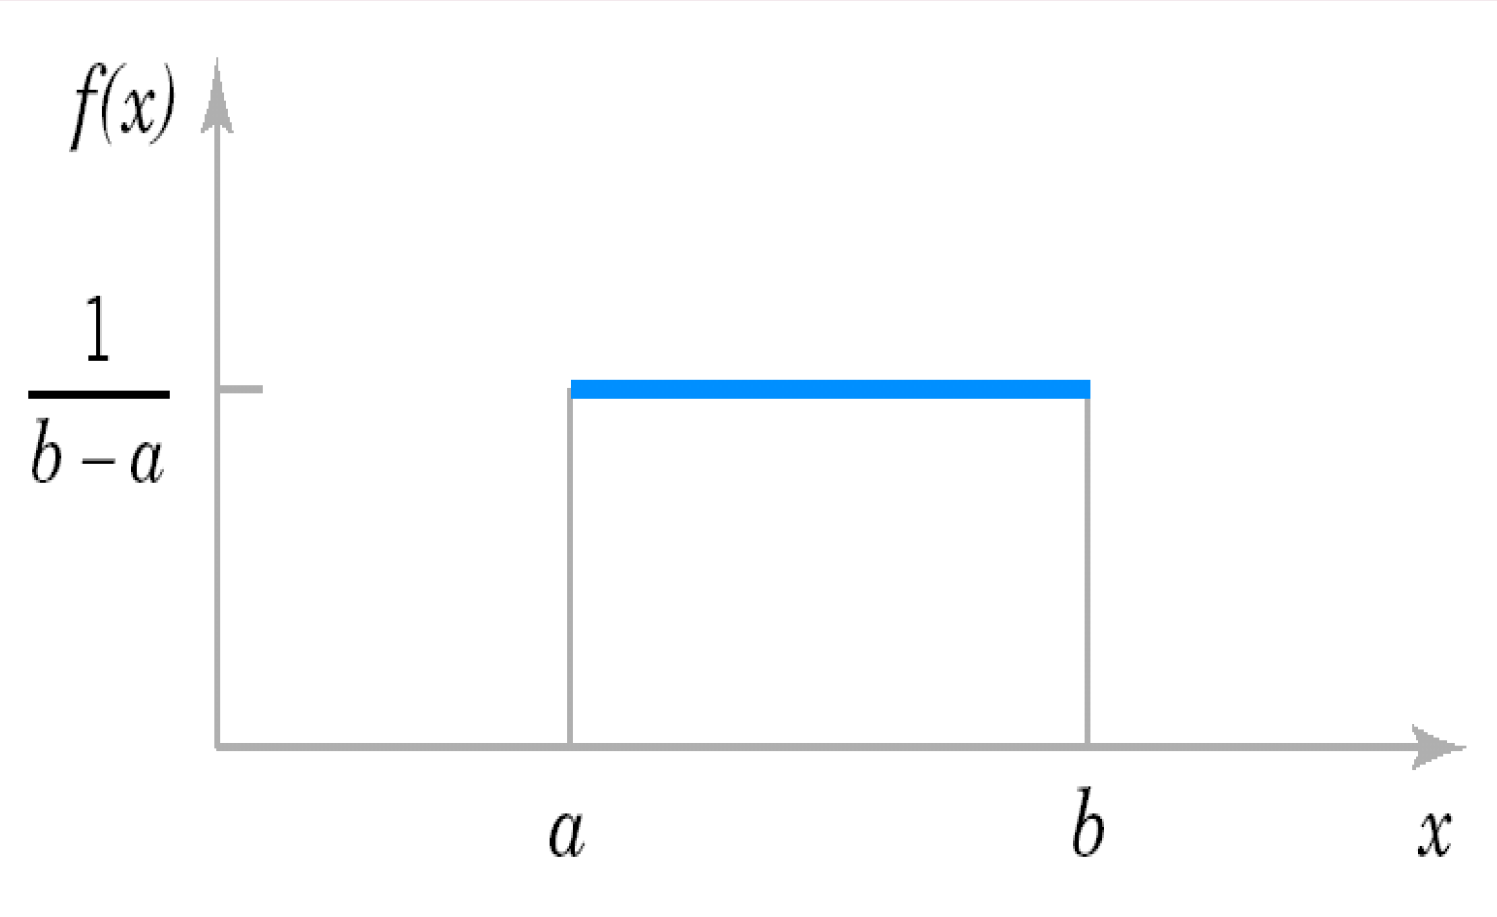
\includegraphics[scale=.12]{figs/Unif_density.png}
 }}
\end{minipage} %
}


\end{frame}








\begin{frame}
\qBrd[4.6in]{ceil!50}{
\begin{center}
Let $X\sim \text{Uniform}(a,b)$ for $a<b$
\end{center}
}\\
\vspace{.5in}

%\qBrd[4.6in]{babyblue!40}{
$\Row{\qBrd[.9in]{amethyst!50}{\text{Mean}\\
\HLTW{E(X)=  \frac{a+b}{2}} \vspace{.2in}},  \qBrd[1.5in]{amethyst!50}{\text{Variance}\\\HLTW{\text{VAR}(X)= \frac{(b-a)^2}{12}   }\vspace{.2in}}  , \qBrd[1.9in]{amethyst!50}{\text{MGF}\\\HLTW{\text{M}_{_X}(t)=\begin{cases} 
 \frac{e^{tb}- e^{ta}}{t(b-a)} & \text{ if } t\neq 0 \\
 1 & \text{ if } t= 0  
 \end{cases} }} } $
%}

\vspace{.1in}
\qBrd[4.75in]{antiquefuchsia!50}{
\begin{center}
\qBrd[4.65in]{white!40}{
{
\tiny
\begin{tabular}{|c|c|c|c|c|c|}
\hline
 Distribution & Support  &  pdf    & Mean   &  Variance  & mgf   \\
& $\support[X]$  &   $f_{_X}(x)$   &  $E(X)$  &   $\text{Var}(X)$  &  $M_{_X}(t)$  \\
 \hline \hline
 & & & & & \\
Uniform$(a,b)$ &$ [a, b]$ & $ f(x)=\begin{cases} \frac{1}{b-a} & \text{ if } x\in [a,b]\\ 0 & \text{ otherwise .} \end{cases} $ & $  \frac{a+b}{2}  $  & $  \frac{(b-a)^2}{12}$&   $M_{_X}(t)
=\begin{cases} 
 \frac{e^{tb}- e^{ta}}{t(b-a)} & \text{ if } t\neq 0 \\
 1 & \text{ if } t= 0  
 \end{cases}$\\
 & & & & & \\
 \hline
  \hline
\end{tabular}
}}\end{center}}
\end{frame}






\begin{frame}
\vspace{-.01in}
\qbx[4.6in]{apricot!40}{
\Exmpl{apricot}{} The time (in min) for a lab assistant to prepare the equipment for a certain experiment is believed to have a uniform distribution with a = 25 and b = 35.
\begin{enumerate}[a).]
\item Write the pdf of X and sketch its graph.
\item What is the probability that preparation time exceeds 33 min?
\item What is the probability that preparation time is within 2 minmutes of the {\bf mean time}?
\end{enumerate}
}\\
\vspace{2.1in}

\end{frame}







\begin{frame}\frametitle{Example}
\tiny
\vspace{-.1in}
\qbx[4.6in]{apricot!40}{
\Exmpl{apricot}{} The time (in min) for a lab assistant to prepare the equipment for a certain experiment is believed to have a uniform distribution with a = 25 and b = 35.
\begin{enumerate}[a).]
\item Write the pdf of X and sketch its graph.
\item What is the probability that preparation time exceeds 33 min?
\item What is the probability that preparation time is within 2 minmutes of the {\bf mean time}?
\end{enumerate}
}\\
%\pause
{\tiny 
\begin{minipage}{.33\textwidth} %
{\tiny 
 \qBrd[1.6in]{babyblue!40}{\begin{center}
 $$\HLTW{ f(x):= \begin{cases} 
 \frac{1}{10}& \text{ if } 25 \leq x\leq 35\\
0 & \text{ otherwise.} 
\end{cases} }$$
 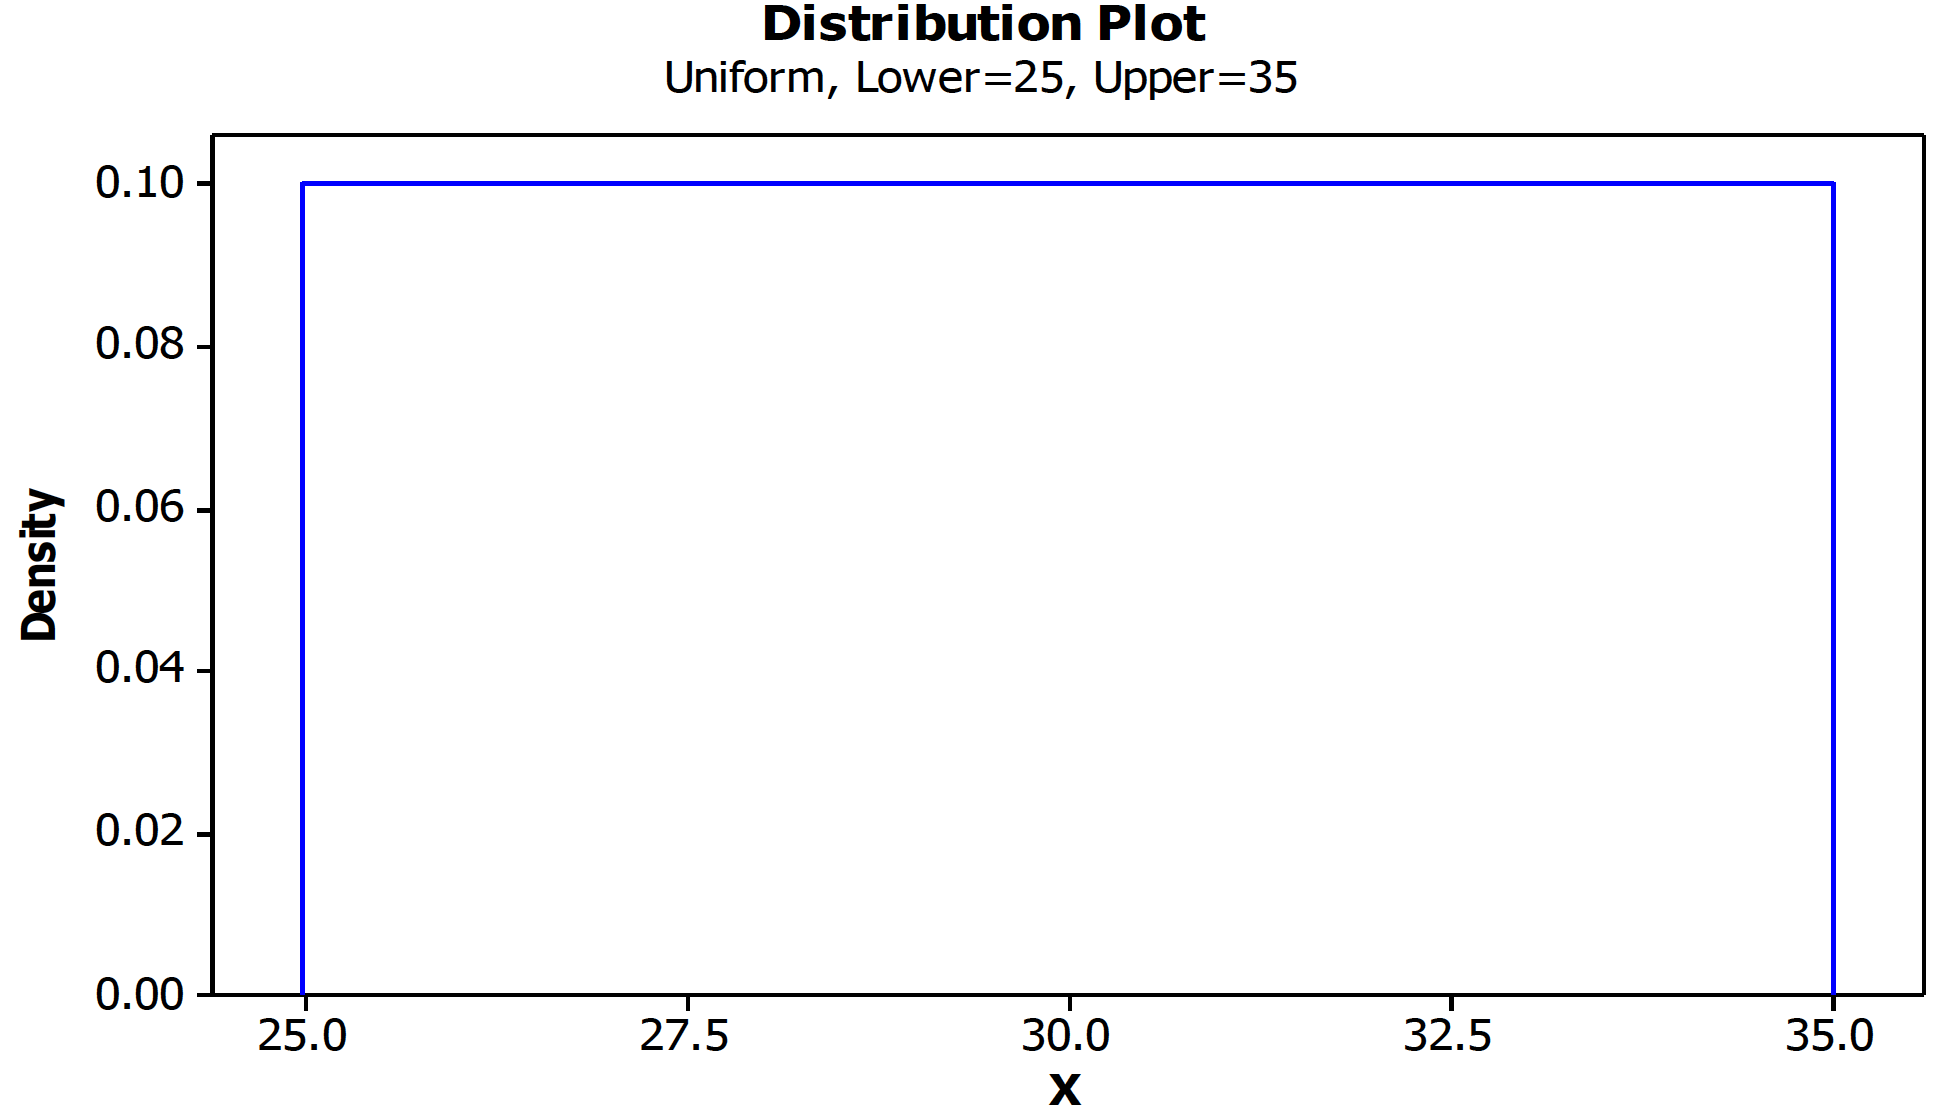
\includegraphics[scale=.1]{figs/Unif_densityExample.png}
 \end{center}
 }
 }
\end{minipage}
\hspace{.1in}
\begin{minipage}{.21\textwidth} %
{\tiny 
 \qBrd[1in]{babyblueeyes!40}{
 \begin{eqnarray}
& &  P(X>33)\nonumber\\
 & = &  \int_{33}^{35} f(x) dx\nonumber\\
& = &  (\frac{x}{10})\Big \vert_{33}^{35}\nonumber\\
 & =&  \frac{35-32}{10}\nonumber\\
  & =&0.2\nonumber
 \end{eqnarray}
 }}
\end{minipage} %
\hspace{.1in}
\begin{minipage}{.38\textwidth} %
{\tiny 
 \qBrd[1.85in]{babyblueeyes!40}{
 Mean of the random variable is\\ $\HLTW{E(X)}= \frac{25+35}{2}= \HLTW{30}$.
 \begin{eqnarray}
& &  P\left(\HLTW{E(X)}-2<X<\HLTW{E(X)}+2\right)\nonumber\\
 & = &   P(30-2<X<30+2)\nonumber\\
& = &   P(28<X<32)\nonumber\\
& = &  \int_{28}^{32} f(x) dx\nonumber\\
& = & \left(\frac{x}{10}\right)\Big \vert_{28}^{32}\nonumber\\
 & =&  \frac{32-28}{10}\nonumber\\
  & =&0.4\nonumber
 \end{eqnarray}
 }}
\end{minipage}

 
}
\end{frame}






\begin{frame}\frametitle{Exercise}
%\tiny
\vspace{-.1in}
\qbx[4.6in]{amethyst!40}{
\Exmpl{amethyst}{} Upon studying low bids for shipping contracts, a microcomputer company finds that intrastate contracts have low bids that are uniformly distributed between 20 and 25, in units of thousands of dollars.
\begin{enumerate}[a).]
\item Find the probability that the low bid on the next intrastate shippingcontract is below \$22,000.
\item Find the probability that the low bid on the next intrastate shipping contract is in excess of \$24,000.
\item Find the expected value and standard deviation of low bids on
contracts of the type described above.
\end{enumerate}
}\\
%\pause
\vspace{2in}
\end{frame}



\begin{frame}\frametitle{Exercise}
%\tiny
\vspace{-.1in}
\qbx[4.6in]{babyblue!40}{
\Exmpl{babyblue}{} A grocery store receives delivery each morning at a time that varies uniformly between 5:00 and 7:00 AM.
\begin{enumerate}[a).]
\item Write and sketch the pdf of the delivery arrival.
\item Find the probability that the delivery on a given morning will occur between 5:30 and 5:45 A.M.
\item Find the probability that the time of delivery will be within one-half standard deviation of the expected time.
\end{enumerate}
}\\
%\pause
\vspace{2in}
\end{frame}


\section{Exponential Distribution}
\TransitionFrame[amber]{\Large Exponential Distribution }


\begin{frame}\frametitle{Exponential Distribution: Context}
\begin{enumerate}
\item The exponential distribution is often used to model time (waiting time, interarrival time, hardware lifetime, failure time, etc.).
\item When the number of occurrences of an event follows Poisson
distribution, the time between occurrences follows exponential
distribution.
\end{enumerate}
\end{frame}



\begin{frame}\frametitle{Exponential Distribution}

\define{Exponential Distribution}{
The exponential probability distribution with parameter $\lambda>0$ (called the
 rate parameter) is 
 $$f(x)= 
  \begin{cases}
\lambda e^{-\lambda x} & \text{ if } x>0\\
0 & \text{ otherwise}
 \end{cases}$$
}

%\qBrd{teal!40}{
%If $X\sim $ Exponential($\lambda$) then 
%$E(X) = \frac{1}{\lambda} \text{ and }, \text{Var}(X) = \frac{1}{\lambda^2}$
%}

\end{frame}


\begin{frame}
\qBrd{applegreen!40}{
The cdf of the exponential distribution is 
$$F(x)= 
  \begin{cases}
  0 & \text{ if } x<0\\
 1- e^{-\lambda x} & \text{ if } x>0
 \end{cases}$$
}
\vspace{2in}
\end{frame}



\begin{frame}
\qBrd[4.6in]{ceil!50}{
\begin{center}
Let $X\sim \text{Exponential}(\HLTW{\text{rate}}= \lambda)$ for $\lambda>0$
\end{center}
}\\
\vspace{.5in}

%\qBrd[4.6in]{babyblue!40}{
$\Row{\qBrd[.9in]{amethyst!50}{\text{Mean}\\
\HLTW{E(X)=  \frac{1}{\lambda} } \vspace{.2in}},  \qBrd[1.5in]{amethyst!50}{\text{Variance}\\\HLTW{\text{VAR}(X)= \frac{1}{\lambda^2}  }\vspace{.2in}}  , \qBrd[1.8in]{amethyst!50}{\text{MGF}\\\HLTW{\text{M}_{_X}(t)=
 \frac{\lambda}{\lambda-t}  \text{ if } 0\leq  t < \lambda } \vspace{.2in}} } $
%}

\vspace{.1in}
\qBrd[4.75in]{antiquefuchsia!50}{
\begin{center}
\qBrd[4.65in]{white!40}{
{
\tiny
\begin{tabular}{|c|c|c|c|c|c|}
\hline
 Distribution & Support  &  pdf    & Mean   &  Variance  & mgf   \\
& $\support[X]$  &   $f_{_X}(x)$   &  $E(X)$  &   $\text{Var}(X)$  &  $M_{_X}(t)$  \\
 \hline \hline
 & & & & & \\
 $\text{Exponential}(\HLTW{\text{rate}}= \lambda)$&$ (0, \infty)$ & $ f(x)=\begin{cases} \lambda e^{-\lambda x} & \text{ if } x>0\\ 0 & \text{ otherwise .} \end{cases} $ & $ \frac{1}{\lambda} $  & $ \frac{1}{\lambda^2}$&   $
 \frac{\lambda}{\lambda-t}  \text{ if } 0\leq  t < \lambda$\\
 & & & & & \\
 \hline
  \hline
\end{tabular}
}}\end{center}}
\end{frame}




\begin{frame}\frametitle{Example}
\vspace{-.1in}
\qbx[4.6in]{apricot!40}{
\Exmpl{apricot}{} Suppose that a study of a certain computer system reveals that the response time, in seconds, has an exponential distribution with a mean of 3 seconds. What is the probability that response time exceeds 5 seconds?
}\\
\vspace{1.8in}
\end{frame}


\begin{frame}\frametitle{Example}
\tiny
\vspace{-.1in}
\qbx[4.6in]{apricot!40}{
\Exmpl{apricot}{} Suppose that a study of a certain computer system reveals that the response time, in seconds, has an exponential distribution with a mean of 3 seconds. What is the probability that response time exceeds 5 seconds?
}\\
%\pause
{\tiny 
\begin{minipage}{.62\textwidth} %
{\tiny 
 \qBrd[2.7in]{babyblue!40}{\begin{center}
 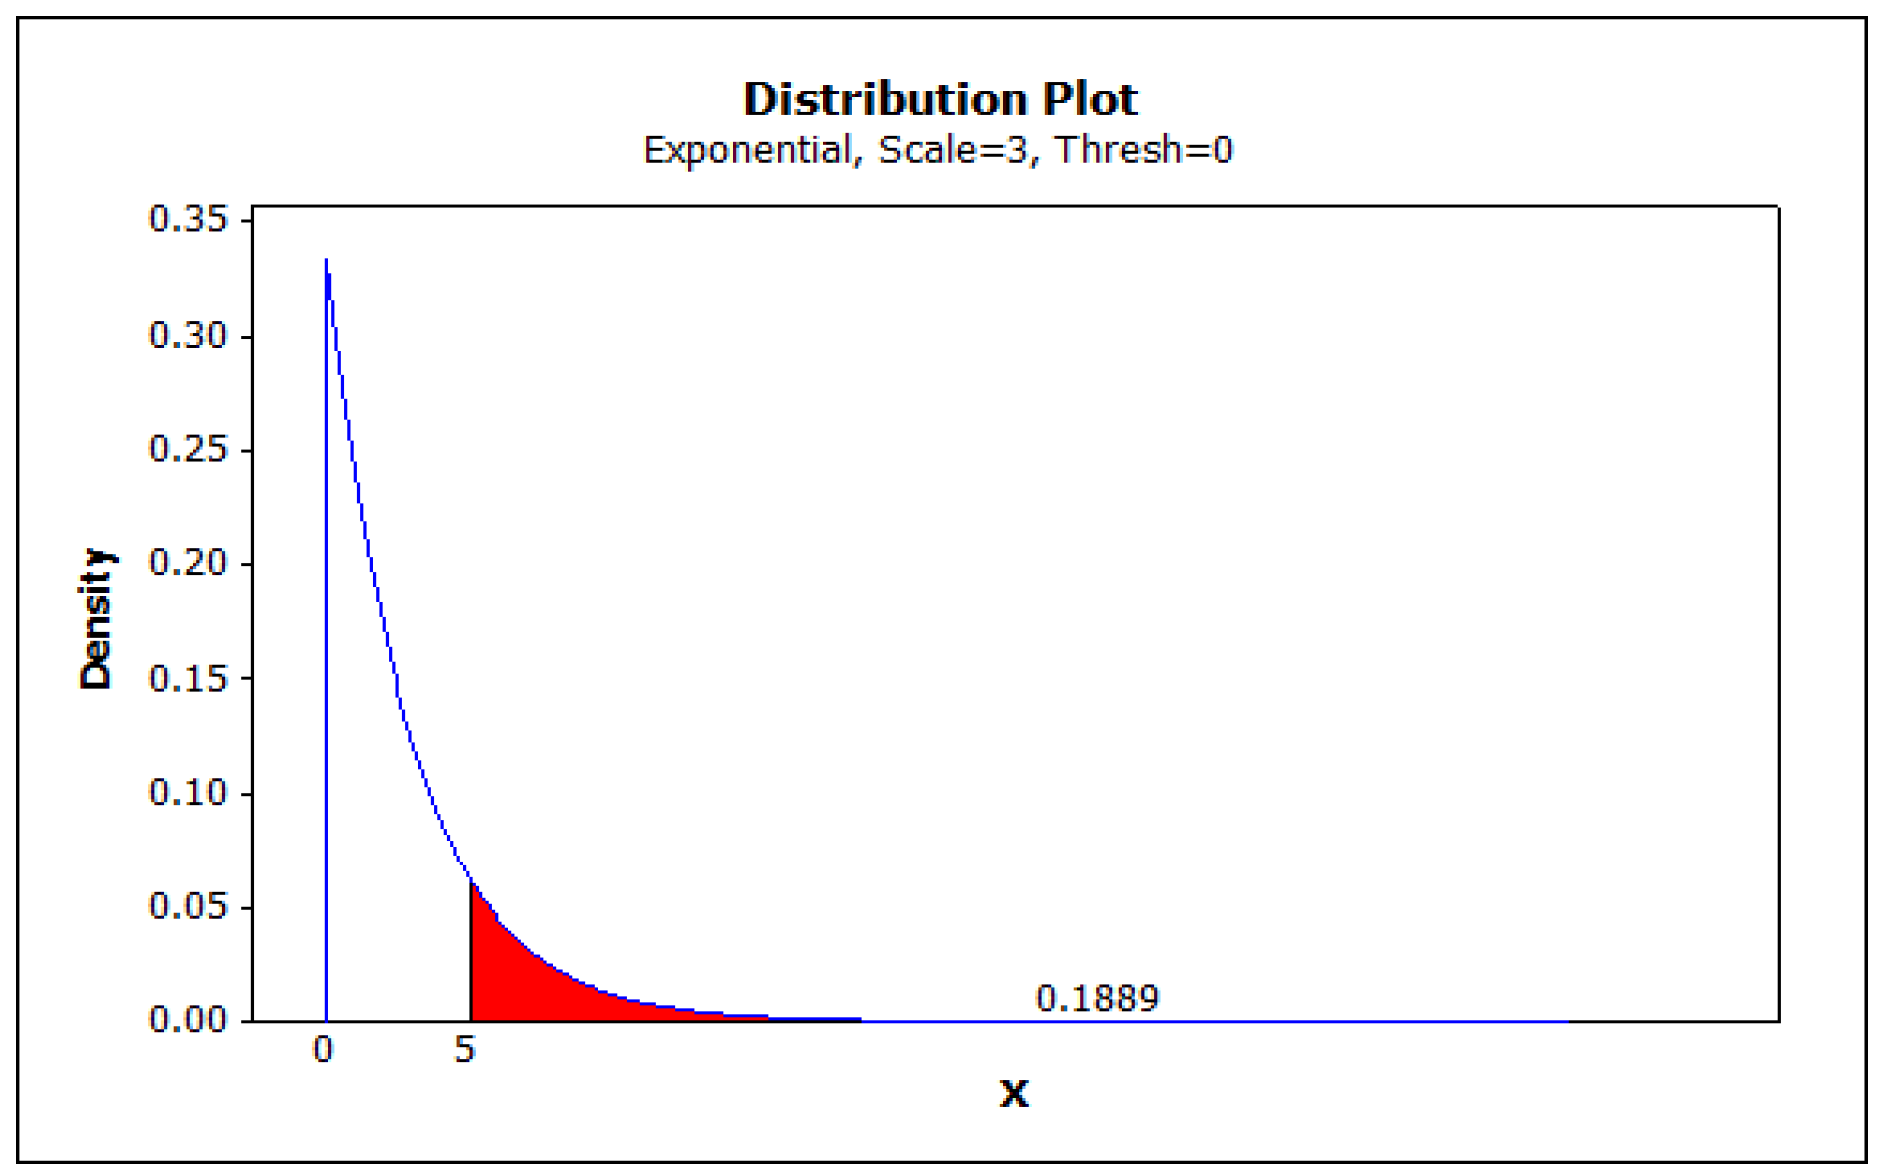
\includegraphics[scale=.2]{figs/pdf_Exponential_density2.png}
 \end{center}
 }
 }
\end{minipage}
\hspace{.1in}
\begin{minipage}{.34\textwidth} %
{\tiny 
 \qBrd[1.4in]{babyblueeyes!40}{
 \begin{eqnarray}
& &  P(X>5)\nonumber\\
 & = &1-P(X\leq 5) \nonumber\\
 & = &1-F( 5) \nonumber\\
  & = &1-\left(1- e^{-\lambda 5} \right) \nonumber\\
   & = & e^{-5\lambda }  \nonumber\\
   & = & e^{-5\times \frac{1}{3} }  \nonumber\\
   & =& 0.1889 \nonumber
 \end{eqnarray}
 }}
\end{minipage} %


 
}
\end{frame}






\begin{frame}\frametitle{Exercise}
%\tiny
\vspace{-.1in}
\qbx[4.6in]{babyblue!40}{
\Exmpl{babyblue}{} The failure rate for a type of electric light bulb is 0.002 per hour. Under the exponential model,
\begin{enumerate}[a).]
\item Find the probability that a randomly selected light bulb will fail in less than 1000 hours.
\item  Find the probability that a randomly selected light bulb will last 2000
hours before failing.
\item Find the mean and the variance of time until failure.
\item  Find the median time until failure.
\item Find the time where 95\% of these bulbs are expected to fail before it.
\end{enumerate}
}\\
%\pause
\vspace{2in}
\end{frame}





\begin{frame}\frametitle{Exercise}
%\tiny
\vspace{-.1in}
\qbx[4.6in]{teal!40}{
\Exmpl{teal}{} An engineer thinks that the best model for time between breakdowns of a generator is the exponential distribution with a mean of 15 days.
\begin{enumerate}[a).]
\item  If the generator has just broken down, what is the probability that it will break down in the next 21 days?
\item What is the probability that the generator will operate for 30 days without a breakdown?
\item If the generator has been operating for the last 20 days, what is the probability that it will operate for another 30 days without a
breakdown?
\item  Comment on the results of parts (b) and (c).
\end{enumerate}
}\\
%\pause
\vspace{2in}
\end{frame}


\section{Gamma Distribution}

\TransitionFrame[bittersweet]{\Large $\HLTW{\Gamma\left(\alpha \right)}$, {\tiny for $\alpha>0$}\\The Gamma Function }


\begin{frame}\frametitle{Gamma Function, $\Gamma(\alpha), \alpha>0$}

 \qBrd[4in]{camel!50}{ \sqBullet{brown}  $\HLTW{ \HLTY{\Gamma\left( \alpha\right)}:= \displaystyle \int\limits_{0}^{\infty}  x^{\alpha-1}e^{-x} dx }$ for $\alpha>0$.}
 
% \begin{itemize}
%\qBrd[2in]{babyblue!40}{ \item  $\HLTY{\Gamma(\alpha)}>0$ for all $\alpha>0$.}
%
%\qBrd[1.6in]{brightube!40}{ \item  $\HLTY{\Gamma(\frac{1}{2})}= \sqrt{\pi}$.}
%
%\qBrd[1in]{cadetgrey!40}{ \item $\HLTY{\Gamma(1)}= 1$}
% \end{itemize}
% \vspace{.3in}
% 
%\begin{itemize}
%\qBrd[3.5in]{applegreen!40}{ \item  $\displaystyle \HLTY{ \Gamma(\alpha)}=\HLTW{ (\alpha-1) \HLTY{\Gamma(\alpha-1)}}$ for any $\HLTW{\alpha>1}$}
%
%\vspace{.05in}
%\qBrd[3.5in]{olive!40}{ \item$\HLTY{\Gamma(n)}= \HLTW{(n-1)!}$ when $n$ is a positive integer.}
%\end{itemize}
\vspace{2in}
\end{frame}


\begin{frame}
\begin{itemize}
\qBrd[2in]{babyblue!40}{ \item[\sqBullet{babyblue}]  $\HLTY{\Gamma(\alpha)}>0$ for all $\alpha>0$.}\\
\vspace{.2in}

\qBrd[1.6in]{brightube!50}{ \item[\sqBullet{brightube}]   $\HLTY{\Gamma(\frac{1}{2})}= \sqrt{\pi}$.}

\qBrd[1in]{cadetgrey!40}{ \item[\sqBullet{cadetgrey}]   $\HLTY{\Gamma(1)}= 1$}
 \end{itemize}
 \vspace{.3in}
 
\begin{itemize}
\qBrd[2.9in]{applegreen!40}{ \item[\sqBullet{applegreen}]  $\displaystyle \HLTY{ \Gamma(\alpha)}=\HLTW{ (\alpha-1) \HLTY{\Gamma(\alpha-1)}}$ for any $\HLTW{\alpha>1}$}

\vspace{.05in}
\qBrd[3.5in]{olive!40}{ \item[\sqBullet{olive}] $\HLTY{\Gamma(n)}= \HLTW{(n-1)!}$ when $n$ is a positive integer.}
\end{itemize}
\end{frame}



\begin{frame}\frametitle{Gamma Function: Example}

 \qBrd[4.7in]{amethyst!40}{   \sqBullet{amethyst}  $\HLTW{  \displaystyle \int\limits_{0}^{\infty}  x^{7}e^{-x} dx }=$ }
 \vspace{.8in}
 
  \qBrd[4.7in]{ceil!40}{   \sqBullet{ceil} $\HLTW{  \displaystyle \int\limits_{0}^{\infty}  x^{\frac{5}{2}}e^{-3x} dx }=$ }

  
   \vspace{1in}
\end{frame}

\begin{frame}\frametitle{Gamma Function: Example}

  \qBrd[4.7in]{olive!40}{   \sqBullet{olive}  $\HLTW{  \displaystyle \frac{\Gamma\left( 9.1\right)}{\Gamma\left( 7.1\right)}}=$ }
   \vspace{1in}
  
   \qBrd[4.7in]{applegreen!40}{ \sqBullet{applegreen}   Let $\alpha>0$,  $\HLTW{  \displaystyle \frac{\Gamma\left( \alpha+3\right)}{\Gamma\left( \alpha\right)}}=$ }
   \vspace{1in}
\end{frame}







\TransitionFrame[amber]{\Large Gamma Distribution }
\begin{frame}
\define{Gamma Distribution}{
The gamma random variable X describes waiting times between
events.  It can be thought of as a waiting time between Poisson
distributed events, the pdf of a Gamma($\alpha, \lambda$) for $\alpha>0, \lambda>0$ is given as:
$$ \HLTW{\displaystyle  f(x)=\frac{\lambda^\alpha}{\Gamma(\alpha)}{ }x^{\alpha-1}e^{-\lambda x}} \text{ for }  0<x<\infty.$$
The parameter $\alpha$ is known as the shape parameter,  while $\lambda$ is called  rate parameter.
}
\vspace{.1in}
\qBrd{applegreen!40}{
Note that: The quantity $\lambda$ is referred to as the  rate parameter.
}\\
\vspace{.1in}
\qBrd{teal!40}{
If $X\sim $ Gamma($\alpha, \lambda$) then 
$E(X) = \frac{\alpha}{\lambda} \text{ and }, \text{Var}(X) = \frac{\alpha}{\lambda^2}$
}
\end{frame}








\begin{frame}
\qBrd[4.6in]{ceil!50}{
\begin{center}
Let $X\sim \text{Gamma}(\HLTW{\text{shape}}= \alpha, \HLTW{\text{rate}}= \lambda)$ for $\alpha>0, \lambda>0$
\end{center}
}\\
\vspace{.5in}

%\qBrd[4.6in]{babyblue!40}{
$\Row{\qBrd[.9in]{amethyst!50}{\text{Mean}\\
\HLTW{E(X)=  \frac{\alpha}{\lambda} } \vspace{.2in}},  \qBrd[1.2in]{amethyst!50}{\text{Variance}\\\HLTW{\text{VAR}(X)= \frac{\alpha}{\lambda^2}  }\vspace{.2in}}  , \qBrd[2in]{amethyst!50}{\text{MGF}\\\HLTW{\text{M}_{_X}(t)=
 \frac{1}{\left( 1-\frac{t}{\lambda}\right)^{\alpha}}  \text{ if } 0\leq  t < \lambda } \vspace{.2in}} } $
%}

\vspace{.1in}
\qBrd[4.75in]{antiquefuchsia!50}{
\begin{center}
\qBrd[4.65in]{white!40}{
{
\tiny
\begin{tabular}{|c|c|c|c|c|c|}
\hline
 Distribution & Support  &  pdf    & Mean   &  Variance  & mgf   \\
& $\support[X]$  &   $f_{_X}(x)$   &  $E(X)$  &   $\text{Var}(X)$  &  $M_{_X}(t)$  \\
 \hline \hline
 & & & & & \\
 $\text{Gamma}(\alpha, \lambda )$&$ (0, \infty)$ & $  \frac{\lambda^{\alpha}}{\Gamma(\alpha)} x^{\alpha-1}e^{-\lambda x}  $ & $ \frac{\alpha}{\lambda} $  & $ \frac{\alpha}{\lambda^2}$&   $ \frac{1}{\left( 1-\frac{t}{\lambda}\right)^{\alpha}}  \text{ if } 0\leq  t < \lambda$\\
 $\HLTW{\text{shape}= \alpha, \text{rate}}= \lambda$ & & $\text{ if } x>0$ & & & \\
 \hline
  \hline
\end{tabular}
}}\end{center}}
\end{frame}




\begin{frame}\frametitle{Exercise}
%\tiny
\vspace{-.1in}
\qbx[4.6in]{babyblue!40}{
\Exmpl{babyblue}{} Suppose the time spent by a randomly selected student who uses a terminal connected to a local time-sharing computer facility has a gamma distribution with mean 20 min and variance 80 min$^2$.
\begin{enumerate}[a).]
\item What are the values of $\alpha$ and $\lambda$?
\item  What is the probability that a student uses the terminal for at most 24 min?
\item What is the probability that a student spends between 20 and 40 min using the terminal?
\end{enumerate}
}\\
%\pause
\vspace{2in}
\end{frame}





\begin{frame}\frametitle{Exercise}
%\tiny
\vspace{-.1in}
\qbx[4.6in]{teal!40}{
\Exmpl{teal}{} A pumping station operator observes that the demand for water at a certain hour of the day can be modeled as an exponential random variable with a mean of 100 cfs (cubic feet per second).
\begin{enumerate}[a).]
\item 1 Find the probability that the demand will exceed 200 cfs on a randomly
selected day.
\item What is the maximum water producing capacity that the station should keep on line for this hour so that the demand will have a probability of only 0.01 of exceeding this production capacity?
\end{enumerate}
}\\
%\pause
\vspace{2in}
\end{frame}





\section{Beta Distribution}


\begin{frame}\frametitle{Beta Function, $\mathscr{B}(\alpha, \beta), \alpha>0, \beta>0$}
\qBrd[4.7in]{babyblueeyes!50}{\sqBullet{babyblue} $ \HLTW{\displaystyle \int\limits_{0}^{1}  x^{3}(1-x)^{9} dx=} $}
\vspace{.5in}

 
\vspace{2in}
\end{frame}

\TransitionFrame[bittersweet]{\Large $\HLTW{\mathscr{B}\left(\alpha, \beta \right)} ${\tiny $\alpha>0, \beta>0$}\\The Beta Function }


\begin{frame}\frametitle{Beta Function, $\mathscr{B}(\alpha, \beta), \alpha>0, \beta>0$}
\begin{center}
\qBrd[4.6in]{cadmiumorange!50}{ $\HLTW{\HLTY{\mathscr{B}\left(\alpha, \beta\right)}:= \displaystyle \int\limits_{0}^{1}  x^{\alpha-1}(1-x)^{\beta-1} dx} $ for $\alpha>0, \beta>0$.}
 \vspace{.1in}
 
 \qBrd[3.8in]{asparagus!50}{
 $ \mathscr{B}\left(\alpha, \beta\right)$ is often calculated using the following equation: 
 $$\HLTW{\displaystyle\HLTY{ \mathscr{B}\left(\alpha, \beta\right)}:= \frac{\Gamma(\alpha)\Gamma(\beta)}{\Gamma(\alpha+\beta)}}$$
 where $\Gamma(\cdot)$ denotes the Gamma function. }
\end{center}
\vspace{2in}
\end{frame}




\begin{frame}\frametitle{Beta Function, $\mathscr{B}(\alpha, \beta), \alpha>0, \beta>0$}
\qBrd[4.7in]{babyblue!50}{  \sqBullet{babyblue}$ \HLTW{\displaystyle \int\limits_{0}^{1}  x^{3}(1-x)^{9} dx=} $}
\vspace{.5in}

\qBrd[4.7in]{celadon!50}{ \sqBullet{celadon}  $ \HLTW{\displaystyle \int\limits_{0}^{1}  x^{30}(1-x)^{1.2} dx=} $}
 
\vspace{2in}
\end{frame}




\TransitionFrame[amber]{\Large Beta Distribution }

\begin{frame}\frametitle{Beta Distribution}
The beta random variable X represents the proportion or probability
outcomes. For example, the beta distribution might be used to find
how likely it is that the preferred candidate for mayor will receive 70\% of the vote.
\define{Beta Distribution}{
Probability Density Function of the Beta($\alpha, \beta$), $\alpha>0, \beta>0$  is given as  
$$  \HLTW{\displaystyle f(x)=\frac{\Gamma(\alpha+\beta)}{\Gamma(\alpha)\Gamma(\beta)} x^{\alpha-1}(1-x)^{\beta-1}}\text{ for }  0\leq x\leq 1., $$
where  $\Gamma(\alpha)$ is defined by $\Gamma(\alpha)= \int_{0}^{\infty} x^{\alpha-1}e^{-x} dx$.
}
\vspace{.1in}
\qBrd{teal!40}{
If $X\sim $ Beta($\alpha, \beta$) then 
$\HLTW{E(X) = \frac{\alpha}{\alpha+\beta} } \text{ and }, \HLTW{\text{Var}(X) = \frac{\alpha \beta}{ (\alpha+\beta)^2(\alpha+\beta+1)}}$
}
\vspace{.5in}
\end{frame}






\begin{frame}
\qBrd[4.6in]{ceil!50}{
\begin{center}
Let $\HLTW{X\sim \text{Beta}(\alpha, \beta)}$ for $\HLTW{\alpha>0, \beta>0.}$
\end{center}
}\\
\vspace{.5in}

%\qBrd[4.6in]{babyblue!40}{
$\Row{\qBrd[.9in]{amethyst!50}{\text{Mean}\\
\HLTW{E(X)=  \frac{\alpha}{\alpha+\beta} } \vspace{.2in}},  \qBrd[1.73in]{amethyst!50}{\text{Variance}\\\HLTW{\text{VAR}(X)=  \frac{\alpha \beta}{ (\alpha+\beta)^2(\alpha+\beta+1)}  }\vspace{.2in}}  , \qBrd[1.5in]{amethyst!50}{\text{MGF}\\\HLTW{\text{M}_{_X}(t)=\text{\tiny A Complicated Series } } \vspace{.2in}} } $
%}

\vspace{.1in}
\qBrd[4.75in]{antiquefuchsia!50}{
\begin{center}
\qBrd[4.65in]{white!40}{
{
\tiny
\begin{tabular}{|c|c|c|c|c|c|}
\hline
 Distribution & Support  &  pdf    & Mean   &  Variance  & mgf   \\
& $\support[X]$  &   $f_{_X}(x)$   &  $E(X)$  &   $\text{Var}(X)$  &  $M_{_X}(t)$  \\
 \hline \hline
 & & & & & \\
 $\text{Beta}(\alpha, \beta )$&$ (0, 1)$ & $   \frac{\Gamma(\alpha+\beta)}{\Gamma(\alpha)\Gamma(
 \beta)}x^{\alpha-1}x^{\beta-1}  $ & $\frac{\alpha}{\alpha+\beta}  $  & $ \frac{\alpha \beta}{ (\alpha+\beta)^2(\alpha+\beta+1)} $&   $ --- $\\
 $\HLTW{\text{shape1}= \alpha, \text{shape2}}= \beta$ & & $\text{ if } 0<x<1$ & & & \\
 \hline
  \hline
\end{tabular}
}}\end{center}}
\end{frame}








\begin{frame}\frametitle{Exercise}
%\tiny
\vspace{-.1in}
\qbx[4.6in]{babyblue!40}{
\Exmpl{babyblue}{} A gasoline wholesale distributor has bulk storage tanks that hold fixed supplies and
are filled every Monday. Of interest to the wholesaler is the proportion of this supply
that is sold during the week. Over many weeks of observation, the distributor found
that this proportion could be modeled by a beta distribution with $\alpha = 4$ and $\beta = 2$.\\
\begin{enumerate}
\item Find the probability that the wholesaler will sell at least 90\% of her stock in a given week.
\item What is the expected percentage of sell in a randomly selected week. 
\end{enumerate}
}\\
%\pause
\vspace{2in}
\end{frame}







\section{Normal Distribution}
\TransitionFrame[amber]{\Huge Normal Distribution }



\TransitionFrame[antiquefuchsia]{\Large Questions?  }
 
 
\end{document}
